\documentclass{IEEEtran}
\usepackage[utf8]{inputenc}
%\usepackage{fullpage}

\usepackage{amsmath}
\usepackage{graphicx}
\usepackage[colorinlistoftodos]{todonotes}
\usepackage[colorlinks=true, allcolors=blue]{hyperref}
\usepackage{mathtools}
\usepackage{latexsym}

\title{MeasureMesh: An Open Source Hardware/Software Platform for Flexible Data Logging}
\author{Matt Ruffner}
\date{}
\begin{document}

\maketitle

%%%%%%%%% ABSTRACT
% \begin{abstract}
% hello
% \end{abstract}



%%%%%%%%%%%%%%%%%%%%%%%%%%%%%
%%%%%%%%%%%%%%%%%%%%%%%%%%%%%
%%%%%%%%%%%%%%%%%%%%%%%%%%%%%
%%%%%%%%%%%%%%%%%%%%%%%%%%%%%
\section{Introduction}
 The Lora Alliance is a not profit association promoting the adoption of a Low Power Wide Area Network (LPWAN) IoT standard knows as Long Range WAN (LoRaWAN). It is a viable platform for low bandwidth, low power remote sensing applications. Over 100 complying companies adopt hardware standards including adaptive bitrate and encryption schemes specific to the LoRaWAN protocol.
 
LoRaWAN is commonly utilized for remote sensing applications including environmental and livestock monitoring~\cite{WuFan2018WAwI,IkhsanMukhammadGufron2018MLGf}. The LoRa standard is designed to be a low power solution, with longer range than traditional wireless means of communication (WiFi, Bluetooth, Zigbee, Z-Wave, etc.). It follows that compared to other wireless protocols, LoRa has significantly lower bandwidth and throughput~\cite{WuFan2018WAwI}. Performance measurements of certain LoRa chipsets have concluded that longer ranges are acheivable in a rural setting with the lowest data rates, and that range in urban settings is less, requiring lower data rates at shorter distances than in rural settings~\cite{RamonSanchez-Iborra2018PEoL}. This suggests that dynamic tuning of the radio parameters is necessary based on deployment location. 

MeasureMesh builds on this LPWAN technology to providing a simple, adaptable hardware and software platform that facilitates easy adoption for custom remote sensing networks. By using off the shelf radios and control units for node and gateway hardware, quick time-to-implementation is acheived, allowing for more focus and customization on sensing needs. The gateway utilizes internet protocol for communicating with a server back-end. For the purposes of this paper, a simple sensor data storage back-end and plotting front-end will be implemented.
%%%%%%%%%%%%%%%%%%%%%%%%%%%%%
%%%%%%%%%%%%%%%%%%%%%%%%%%%%%
%%%%%%%%%%%%%%%%%%%%%%%%%%%%%
%%%%%%%%%%%%%%%%%%%%%%%%%%%%%
\section{Project Overview} 

MeasureMesh consists of numerous nodes talking to a gateway which in turn logs collected data to a cloud databse via internet.

project consists of one or many nodes, nodes have same hardware, reconfigure node address in software. sen

\begin{figure}[h!]
    \centering
    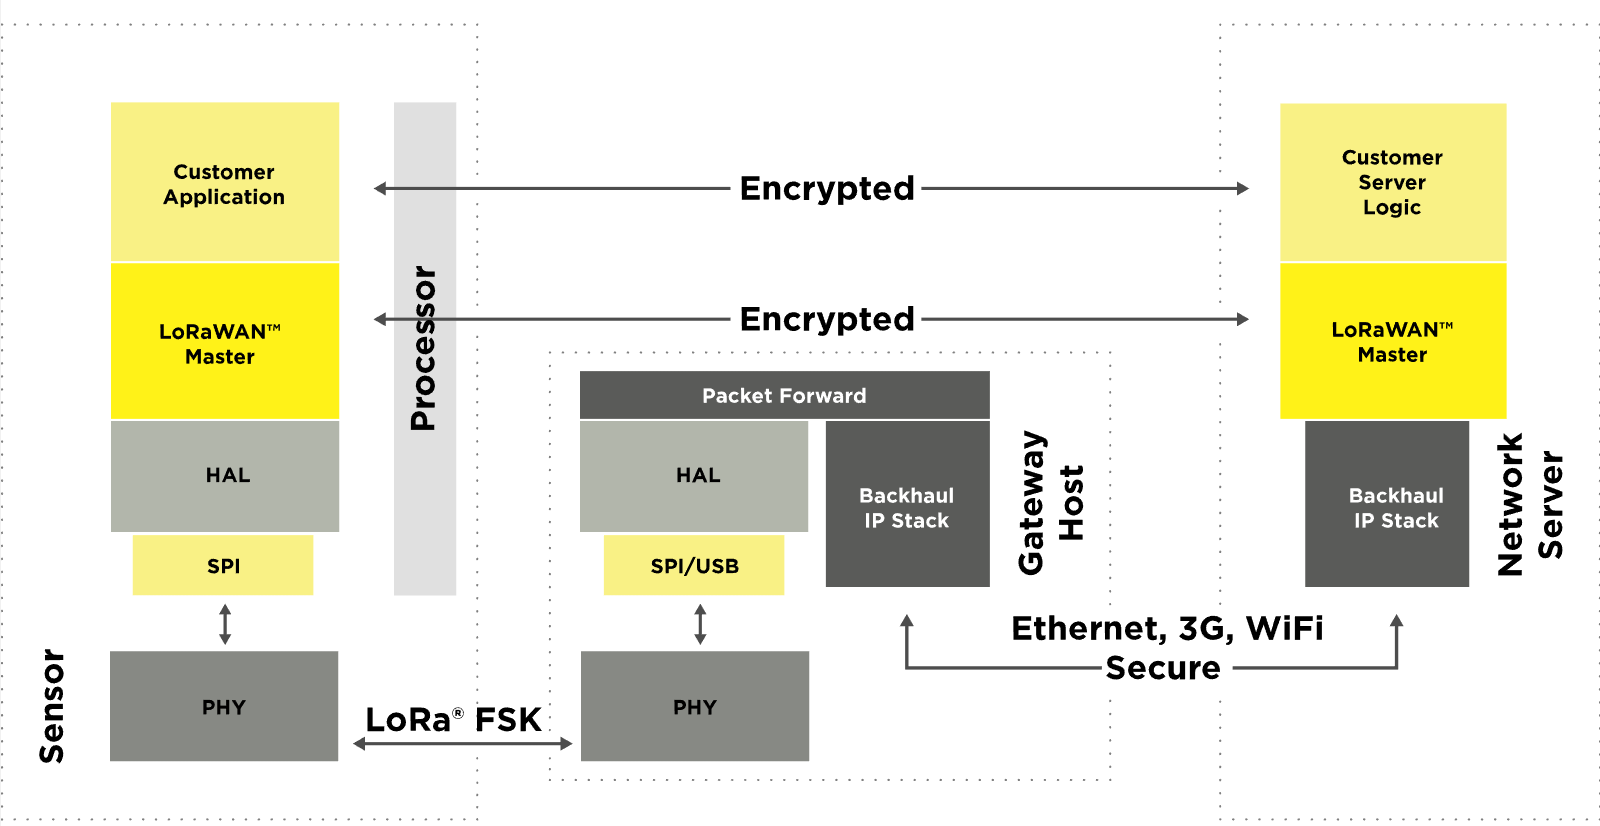
\includegraphics[width=8cm]{images/lorasystem}
    \caption{LoRa network overview.}
    \label{fig:lora_overview}
\end{figure}


Describe the overall functionality along with the constituent modules of your project, as envisioned in the final product. Clearly describe different hardware and software parts/modules used or to be used. Use block diagrams, concept diagrams, graphs, flow-charts, algorithms, demo pictures, etc., to aid your description when appropriate.

%%%%%%%%%%%%%%%%%%%%%%%%%%%%%
%%%%%%%%%%%%%%%%%%%%%%%%%%%%%
%%%%%%%%%%%%%%%%%%%%%%%%%%%%%
%%%%%%%%%%%%%%%%%%%%%%%%%%%%%
\section{Projected Task Schedule} 
Divide your project into deliverable tasks and briefly describe the goals and outcomes of each task. For each task, describe an estimated timeline and workload division (in case of group projects). Clearly distinguish completed tasks from to-do tasks.

%%%%%%%%%%%%%%%%%%%%%%%%%%%%%
%%%%%%%%%%%%%%%%%%%%%%%%%%%%%
%%%%%%%%%%%%%%%%%%%%%%%%%%%%%
%%%%%%%%%%%%%%%%%%%%%%%%%%%%%
\section{Learning Outcome}

What new did you learn for this project? Describe.



\bibliographystyle{ieeetr}
\bibliography{refs.bib}

\end{document}
